\documentclass[twoside,11pt]{article}

% Any additional packages needed should be included after jmlr2e.
% Note that jmlr2e.sty includes epsfig, amssymb, natbib and graphicx,
% and defines many common macros, such as 'proof' and 'example'.
%
% It also sets the bibliographystyle to plainnat; for more information on
% natbib citation styles, see the natbib documentation, a copy of which
% is archived at http://www.jmlr.org/format/natbib.pdf

\usepackage{jmlr2e}
\usepackage{graphicx}% Definitions of handy macros can go here
\usepackage{hyperref}


% Heading arguments are {volume}{year}{pages}{submitted}{published}{author-full-names}

\jmlrheading{1}{2009}{1-4}{2/09}{10/09}{Brian Tanner and Adam White}

% Short headings should be running head and authors last names

\ShortHeadings{RL-Glue}{Tanner and White}
\firstpageno{1}

\begin{document}

\title{RL-Glue : Language-Independent Software for Reinforcement-Learning Experiments}


\author{\name Brian Tanner \AND Adam White  \email \{btanner,awhite\}@cs.ualberta.ca \\
       \addr Department of Computing Science, University of Alberta, Canada}

\editor{ Soeren Sonnenburg}

\maketitle

\begin{abstract}
RL-Glue is a standard, language-independent software package for reinforcement-learning experiments.  The standardization provided by RL-Glue facilitates code sharing and collaboration.  Code sharing reduces the need to re-engineer tasks and experimental apparatus, both common barriers to comparatively evaluating new ideas in the context of the literature.  Our software features a minimalist interface and works with several languages and computing platforms. RL-Glue compatibility can be extended to any programming language that supports network socket communication. RL-Glue has been used to teach classes, to run international competitions, and is currently used by several other open-source software and hardware projects.
\end{abstract}

\section{Introduction and Motivation}
\vspace{-0.2cm}
Reinforcement learning is an embodied, trial-and-error problem formulation for artificial intelligence~\citep{rlbook, rlsurvey,ndp}.  At a series of time steps, the {\it agent} emits actions in response to observations and rewards that have been generated by the {\it environment}.  The agent's objective is to select actions that maximize the future rewards.  Reinforcement-learning methods have been successfully applied to many problems including %
%update for final when we get refs automobile traffic flow-control \citep{traffice-ref} and computer Go\citep{go-ref}. 
  backgammon~\citep{tesauro:nc94}, elevator control~\citep{crites:mlj98},
and helicopter control~\citep{ng:iser04}.  
Reinforcement-learning models and formalisms have influenced a number of fields, including operations research, cognitive science, optimal control, psychology, neuroscience, and others.


Reinforcement-learning practitioners create their agents and environments using various incompatible software frameworks, making collaboration inconvenient and thus slowing progress in our community.  It can be time consuming, difficult, and sometimes even impossible to exactly reproduce the work of others.  A conference or journal article is not the appropriate medium to share a sufficiently detailed specification of the environment, agent and overall experimental apparatus.  We need a convenient way to share source code.

We believe that a standard programming interface for reinforcement-learning experiments will remove some barriers to collaboration and accelerate the pace of research in reinforcement learning.  To encourage widespread adoption, this interface should be easy to adhere to, and it should not force users to abandon their favorite tools or languages.  With these goals in mind, we have developed RL-Glue: language independent software for reinforcement-learning experiments.


\vspace{-0.2cm}
\section{RL-Glue}
\vspace{-0.2cm}
Reinforcement-learning environments cannot be stored as fixed data-sets, as is common in conventional supervised machine learning.  The environment generates observations and rewards in response to actions selected by the agent, making it more natural to think of the environment and agent as interactive \textit{programs}.  Sutton and Barto describe one prevalent view of agent-environment interactions in their introductory text\citep{rlbook}.  Their view, shown in Figure \ref{fig:agent-env}, clearly separates the agent and environment into different components which interact in a particular way, following a particular sequence.   

\vspace{-0.4cm}
\begin{figure}[ht]
\begin{center}
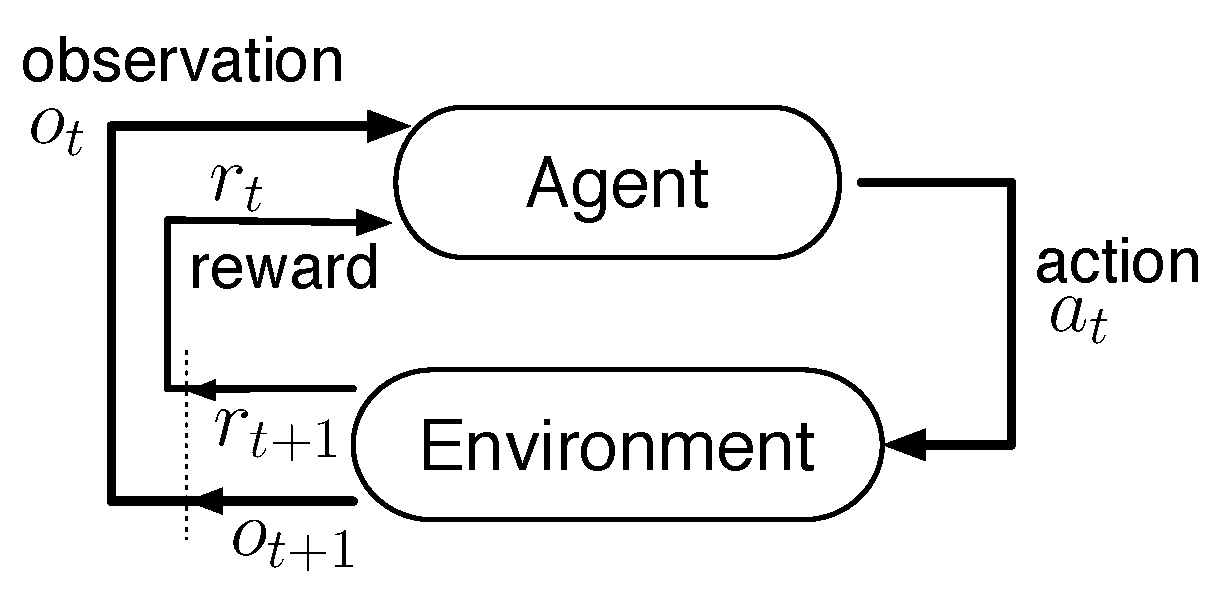
\includegraphics[height=3cm]{figures/agent-env.pdf}
\vspace{-0.4cm}
\caption{\small Sutton and Barto's agent-environment interface, with states generalized to observations.}
\label{fig:agent-env}
\end{center}
\vspace{-0.7cm}
\end{figure}


\citeauthor{whiteThesis}'s RL-Glue Protocol (\citeyear{whiteThesis}) formalizes Sutton and Barto's interface for online, single-agent reinforcement learning.  The RL-Glue Protocol describes how the different aspects of a reinforcement-learning experiment should be arranged into programs, and the etiquette these programs should follow when communicating with each other. These programs (Figure \ref{fig:RLDIA}) are the agent, the environment, the experiment, and RL-Glue.  The agent program contains the learning algorithm and action-selection mechanism. The environment program implements the dynamics of the task and generates the rewards. The experiment program directs the experiment's execution, including the sequence of agent-environment interactions and agent performance evaluation.  The RL-Glue program mediates the communication between the agent and environment programs in response to commands from the experiment program. Our RL-Glue Software (RL-Glue) is an implementation of \citeauthor{whiteThesis}'s RL-Glue Protocol. 

\vspace{-0.4cm}
\begin{figure}[ht]
\begin{center}
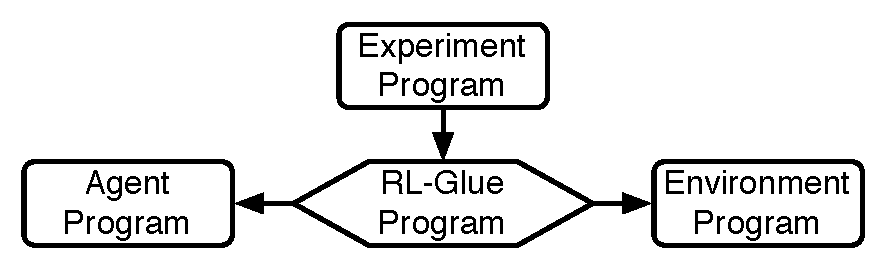
\includegraphics[height=3cm]{figures/glue.pdf}
\vspace{-0.4cm}
\caption{\small The four programs specified by the RL-Glue Protocol.  Arrows indicate the direction of the flow of control.}
\label{fig:RLDIA}
\end{center}
\vspace{-0.7cm}
\end{figure}

 RL-Glue can be used either in  internal or external mode.  In \textit{internal} mode, the agent, environment and experiment are linked into a single program, and their communication is through function calls.  Internal mode is currently an option if the agent, environment, and experiment are written exclusively in Java or C/C++.  In  \textit{external} mode, the agent, environment and experiment are linked into separate programs.  Each program connects to the RL-Glue server program, and all communication is over TCP/IP socket connections. External mode allows these programs to be written in any programming language that supports socket communication.  External mode is currently supported for C/C++, Java, Python, Lisp, and Matlab.

Each mode has its strengths and weaknesses. Internal mode has less overhead, so it can execute more steps per second. External mode is more flexible and portable.  The performance difference between the two modes vanishes as the agent or environment becomes complex such that computation dominates the socket overhead in terms of time per step.  The agent and environment are indifferent and unaware of their execution mode: the difference in modes lies only in how the agent and environment are linked or loaded.

\section{RL-Glue in Practice}
\vspace{-0.2cm}
RL-Glue's common interface has been used by a number of software and hardware projects in the reinforcement-learning community.  For example, there is an annual competition,\footnote{\url{http://www.rl-competition.org/}} where teams from around the world compare their agents on a variety of challenging environments.  The competition software uses an API\footnote{\url{http://code.google.com/p/rl-viz/}} that is layered on top of RL-Glue to dynamically load agent and environment programs, modify parameters at runtime and visualize interaction and performance.  All of the environments and sample agents created by the competition organizers are added to the RL-Library,\footnote{\url{http://library.rl-community.org/}} a public, community-supported repository of RL-Glue compatible code. The RL-Library is also available as a showcase and archive of top competition agents, challenge problems, project code from academic publications, or any other RL-Glue compatible software that members of our community would like to share.


The socket architecture of RL-Glue allows diverse software and hardware platforms to be connected as RL-Glue environment programs.  There are ongoing projects that connect a mobile robot platform,\footnote{\url{http://www.cs.ualberta.ca/~sokolsky/critterbot/}} a  keepaway soccer server, a real-time strategy game, and an Atari emulator to RL-Glue. Our socket architecture helps lower the barriers for researchers wishing to work on larger scale environments by providing a simple and familiar interface. %These environments will soon be accessible via RL-Library. 

RL-Glue has been used for teaching reinforcement learning in several university courses and to create experiments for scientific articles published in leading conferences. We maintain an updated list\footnote{\url{http://glue.rl-community.org/rl-glue-in-practice}} of all known projects that have benefited from RL-Glue.



\vspace{-0.2cm}
\section{Other Reinforcement-Learning Software Projects}
\vspace{-0.2cm}
RL-Glue is not the first software project that aims to  standardize empirical reinforcement learning or to make agent and environment programs more accessible within our community.  However, RL-Glue is the only project that offers a standardized language-independent interface, rich actions and observations, and fine-grained control of the experiment.

Other projects, most notably: CLSquare,\footnote{\url{http://www.ni.uos.de/index.php?id=70}}  PIQLE,\footnote{\url{http://piqle.sourceforge.net/}} RL Toolbox,\footnote{\url{http://www.igi.tugraz.at/ril-toolbox/}
} JRLF,\footnote{\url{http://mykel.kochenderfer.com/jrlf/}}  and LibPG,\footnote{\url{http://code.google.com/p/libpgrl/}} offer significant value to the reinforcement-learning community by offering agents and environments, intuitive visualizations, programming tools, etc.  Users should not be forced to choose between RL-Glue and these alternative projects. Our design makes it relatively easy to interface existing frameworks with RL-Glue.  We are currently offering our assistance in bridging other frameworks to RL-Glue, with the hope of improving access to all of these tools for all members of our community.

 
\vspace{-0.2cm}
\section{RL-Glue Open Source Project}
\vspace{-0.2cm}
\begin{tabular}{ l l}
  \textbf{Website:} \url{http://glue.rl-community.org}  & \textbf{License:} \texttt{Apache 2.0}  \end{tabular}
\newline
\newline
RL-Glue is more than an interface; it connects a family of community projects, with many levels of possible participation. Members of the community are invited to submit agent, environment and experiment programs to the RL-Library. Developers can also extend the reach of RL-Glue compatibility by writing external-mode or internal-mode interfaces for their favorite programming language.  The RL-Glue Software project also welcomes submissions and improvements for all parts of the software and documentation.  

\vspace{-0.2cm}
\section{Acknowledgements}
\vspace{-0.2cm}
We would like to thank the users, testers, and developers for their contributions to RL-Glue 3.0. Special thanks to 
G\'{a}bor Bal\'{a}sz,  %get the accents right
Jos\'{e} Antonio Martin H.,  %get the accents right
Scott Livingston, %Middle Initial?
Marc Bellemare, 
Istv\'{a}n Szita,  %get the accents right
Marc Lanctot, 
Anna Koop, 
Dan Lizotte,
Richard Sutton,
Monica Dinculescu,
Jordan Frank, and
Andrew Butcher.  Of course, we also owe a great debt to all of the talented people responsible for the historic and ongoing development of RL-Glue.\footnote{\url{http://glue.rl-community.org/contributors-history}}

%\addcontentsline{toc}{chapter}{Bibliography}
     %add the above line to get "Bibliography" in the table of contents.
%
%\singlespacing % optional;  Bibliography is better in single spacing
               %            but you may choose different
               %            Don't use \singlespacing if your thesis
               %            is already in single spacing
%
                          % for long bibs.



\bibliographystyle{natbib}
\setlength{\bibsep}{6pt}
\bibliography{jmlrTake2}



\end{document}  
